\documentclass{article} %选择文档类型,我们如果是做期末大作业的话选article就可以了

\usepackage{anyfontsize}
%正如c++需要import库来实现各种各样的功能,Latex也需要调用宏包来实现各种各样的功能
\usepackage{amsmath}  %调用公式宏包
\usepackage{graphicx} %调用插图宏包
\graphicspath{{code_Latex/}}
\usepackage{ctex}     %调用中文宏包
\usepackage{float}
\usepackage{cite}


%\begin{document}这句话之前是导言区,这句话以后就开始写正文了
%可以把导言区理解为int main()函数之前的内容,而正文就是int main()主函数的部分了
\usepackage{geometry}
\geometry{left=1.5cm,right=0.5cm,top=1.0cm,bottom=1.5cm}

\begin{document}
    \title{\centerline{高性能计算实验报告}}
    \date{实验六}
    \author{信息学部 2023311704 王昕远}
    \maketitle
    \thispagestyle{empty}
% \section{硬件配置}% \texttt{ OS版本: Linux wxy 5.15.153.1-microsoft-standard-WSL2 \#1 SMP Fri Mar 29 23:14:13 UTC 2024 x86\_64 x86\_64 x86\_64 GNU/Linux}




% \section{理论峰值计算}

% \includegraphics[width=0.8\textwidth]{1.png}

\section{实验环境}
操作系统版本:Ubantu 22.04.3 LTS\par
CPU型号:AMD Ryzen 7 7745HX with Radeon Graphics 物理核数:8 频率:3600MHz\par

\section{blas}
\begin{verbatim}
void MY_MMult_blas(int m, int n, int k, double *a, int lda,
              double *b, int ldb,
              double *c, int ldc)
{
  cblas_dgemm(CblasRowMajor, CblasNoTrans, CblasNoTrans,    
   m, n, k, 1.0, a, lda, b, ldb, 1.0, c, ldc);
}
    \end{verbatim}
    


\section{pthread}
\begin{verbatim}
    #include <stdio.h>
    #include <omp.h>
    #include "defs.h"
    #include <pthread.h>
    #include <sys/time.h>
    
    #define NUM_THREADS 4  // 定义线程数量
    
    typedef struct {
        double *A;
        double *B;
        double *C;
        int m, n, k;
        int start_row;
        int end_row;
    } thread_data_t;
    
    // 多线程DGEMM计算部分
    void *thread_dgemm(void *arg) {
        thread_data_t *data = (thread_data_t *)arg;
        double *A = data->A;
        double *B = data->B;
        double *C = data->C;
        int m = data->m;
        int n = data->n;
        int k = data->k;
        int start_row = data->start_row;
        int end_row = data->end_row;
    
        for (int i = start_row; i < end_row; i++) {
            for (int j = 0; j < n; j++) {
                double sum = 0.0;
                for (int p = 0; p < k; p++) {
                    sum += A[i * k + p] * B[p * n + j];
                }
                C[i * n + j] = sum;
            }
        }
    
        pthread_exit(NULL);
    }
    
    void MY_MMult_pthread(int m, int n, int k, double *A, int lda, double *B, int ldb, double *C, int ldc) {
        pthread_t threads[NUM_THREADS];
        thread_data_t thread_data[NUM_THREADS];
        int rows_per_thread = m / NUM_THREADS;
    
        // 记录起始时间
        struct timeval start, end;
        gettimeofday(&start, NULL);
    
        // 分配每个线程负责的行
        for (int i = 0; i < NUM_THREADS; i++) {
            thread_data[i].A = A;
            thread_data[i].B = B;
            thread_data[i].C = C;
            thread_data[i].m = m;
            thread_data[i].n = n;
            thread_data[i].k = k;
            thread_data[i].start_row = i * rows_per_thread;
            thread_data[i].end_row = (i == NUM_THREADS - 1) ? m : (i + 1) * rows_per_thread;
    
            pthread_create(&threads[i], NULL, thread_dgemm, (void *)&thread_data[i]);
        }
    
        // 等待所有线程完成
        for (int i = 0; i < NUM_THREADS; i++) {
            pthread_join(threads[i], NULL);
        }
    
        // 记录结束时间
        gettimeofday(&end, NULL);
    
        // 计算时间差
        double time_taken = (end.tv_sec - start.tv_sec) * 1e6;
        time_taken = (time_taken + (end.tv_usec - start.tv_usec)) * 1e-6;
    
        // printf("MY_MMult (多线程) 完成,耗时: %f 秒\n", time_taken);
    }
\end{verbatim}

\section{openMP}
\begin{verbatim}
    #include <stdio.h>
    #include <omp.h>
    #include "defs.h"
    
    void MY_MMult_openmp(int m, int n, int k, double *A, int lda, double *B, int ldb, double *C, int ldc) {
        int i, j, p;
        double sum;
    
        // Parallelized outer loops with OpenMP
        #pragma omp parallel for private(i, j, p, sum) shared(A, B, C)
        for (i = 0; i < m; i++) {
            for (j = 0; j < n; j++) {
                sum = 0.0;
                for (p = 0; p < k; p++) {
                    sum += A[i * lda + p] * B[p * ldb + j];
                }
                C[i * ldc + j] = sum;
            }
        }
    }
    
\end{verbatim}


\section{gflops曲线图}
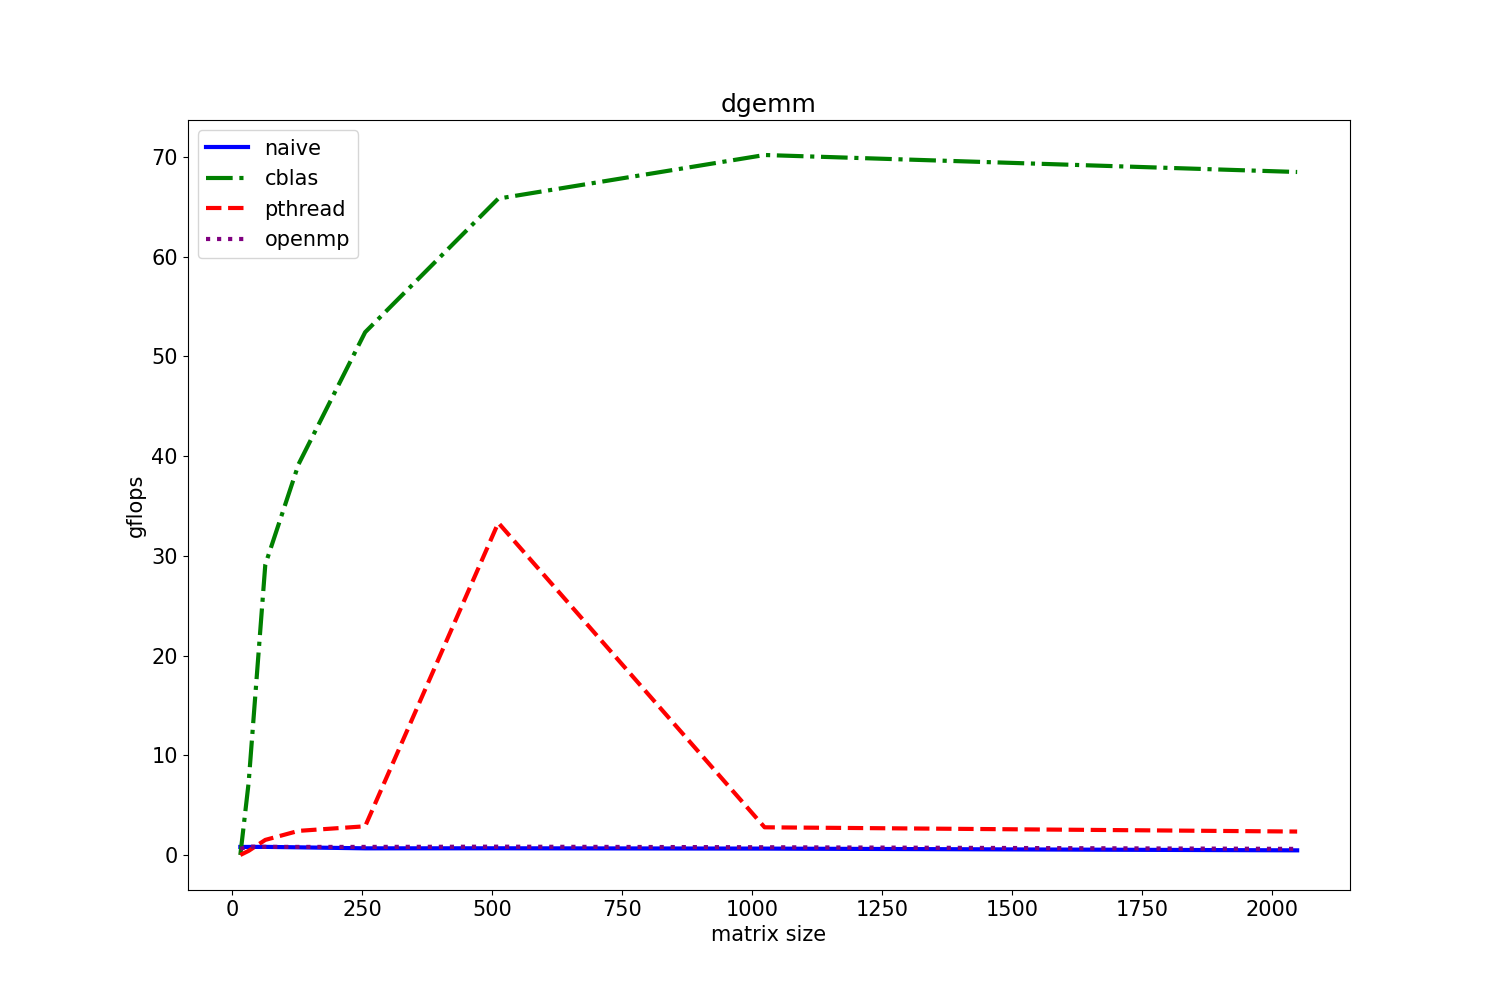
\includegraphics[width=0.8\textwidth]{result.png}
% \section{time-dgemm}
% \begin{tabular}{|c|c|c|c|c|}
%     \hline
%      & time \\ \hline
%     real & 0m38.037s \\ \hline
%     uesr  &1m15.746s \\ \hline
%     system &0m0.220s \\ \hline
%     (real+uesr)/system & 517.195s \\ \hline
% \end{tabular}

$$
$$




\end{document}